%%% File-Information {{{
%%% Filename: thesis_main.tex
%%% Purpose: bachelor thesis
%%%
%%% Notes:
%%%
%%%
%%%
%%% }}}
%%%%%%%%%%%%%%%%%%%%%%%%%%%%%%%%%%%%%%%%%%%%%%%%%%%%%%%%%%%%%%%%%%%%%%%%%%%%%%%%
%%% main document {{{

\documentclass[
a4paper,     %% defines the paper size: a4paper (default), a5paper, letterpaper, ...
% twoside,     %% changes to a two-page-layout (alternatively: oneside)
% headsepline, %% add a horizontal line below the column title
% footsepline, %% add a horizontal line above the page footer
titlepage,   %% only the titlepage (using titlepage-environment) appears on the first page (alternatively: notitlepage)
% parskip,     %% insert an empty line between two paragraphs (alternatively: halfparskip, ...)
% leqno,       %% equation numbers left (instead of right)
% fleqn,       %% equation left-justified (instead of centered)
% tablecaptionabove, %% captions of tables are above the tables (alternatively: tablecaptionbelow)
14pt         %% set default font size to 12 point
]{scrartcl}  %% article, see KOMA documentation (scrguide.dvi)



%%%%%%%%%%%%%%%%%%%%%%%%%%%%%%%%%%%%%%%%%%%%%%%%%%%%%%%%%%%%%%%%%%%%%%%%%%%%%%%%
%%%
%%% packages
%%%

%%%
%%% encoding and language set
%%%

%%% fontenc, ae, aecompl: coding of characters in PDF documents
\usepackage[T1]{fontenc}
\usepackage{ae,aecompl}

%%%
%%% technical packages
%%%

%%% amsmath, amssymb, amstext: support for mathematics
\usepackage{amsmath,amssymb,amstext,amsthm}
\newtheoremstyle{mystyle}%                % Name
  {}%                                     % Space above
  {}%                                     % Space below
  {\itshape}%                                     % Body font
  {}%                                     % Indent amount
  {\bfseries}%                            % Theorem head font
  {.}%                                    % Punctuation after theorem head
  { }%                                    % Space after theorem head, ' ', or \newline
  {\thmname{#1}\thmnumber{ #2}\thmnote{ (#3)}}%                                     % Theorem head spec (can be left empty, meaning `normal')

\theoremstyle{mystyle}
\newtheorem*{definition}{Definition}
\newtheorem*{satz}{Satz}
\newtheorem*{prot}{Protokoll}
\renewcommand*{\proofname}{Beweis}
%\let\oldproofname=\proofname
%\renewcommand*{\proofname}{\rm\bf{\oldproofname}}
%\renewenvironment{proof}{{\bfseries Proof}}{}


%%% psfrag: replace PostScript fonts
\usepackage{psfrag}

%%% listings: include programming code
%\usepackage{listings}

%%% units: technical units
%\usepackage{units}

%%%
%%% layout
%%%

%%% scrpage2: KOMA heading and footer
%%% Note: if you don't use this package, please remove 
%%%       \pagestyle{scrheadings} and corresponding settings
%%%       below too.
\usepackage[automark]{scrpage2}


%%%
%%% PDF
%%%

\usepackage{ifpdf}

%%% Should be LAST usepackage-call!
%%% For docu on that, see reference on package ``hyperref''
\ifpdf%   (definitions for using pdflatex instead of latex)

  %%% graphicx: support for graphics
  \usepackage[pdftex]{graphicx}

  \pdfcompresslevel=9

  %%% hyperref (hyperlinks in PDF): for more options or more detailed
  %%%          explanations, see the documentation of the hyperref-package
  \usepackage[%
    %%% general options
    pdftex=true,      %% sets up hyperref for use with the pdftex program
    %plainpages=false, %% set it to false, if pdflatex complains: ``destination with same identifier already exists''
    %
    %%% extension options
    backref,      %% adds a backlink text to the end of each item in the bibliography
    pagebackref=false, %% if true, creates backward references as a list of page numbers in the bibliography
    colorlinks=true,   %% turn on colored links (true is better for on-screen reading, false is better for printout versions)
    %
    %%% PDF-specific display options
    bookmarks=true,          %% if true, generate PDF bookmarks (requires two passes of pdflatex)
    bookmarksopen=false,     %% if true, show all PDF bookmarks expanded
    bookmarksnumbered=false, %% if true, add the section numbers to the bookmarks
    %pdfstartpage={1},        %% determines, on which page the PDF file is opened
    pdfpagemode=None         %% None, UseOutlines (=show bookmarks), UseThumbs (show thumbnails), FullScreen
  ]{hyperref}


  %%% provide all graphics (also) in this format, so you don't have
  %%% to add the file extensions to the \includegraphics-command
  %%% and/or you don't have to distinguish between generating
  %%% dvi/ps (through latex) and pdf (through pdflatex)
  \DeclareGraphicsExtensions{.pdf}

\else %else   (definitions for using latex instead of pdflatex)

  \usepackage[dvips]{graphicx}

  \DeclareGraphicsExtensions{.eps}

  \usepackage[%
    dvips,           %% sets up hyperref for use with the dvips driver
    colorlinks=false %% better for printout version; almost every hyperref-extension is eliminated by using dvips
  ]{hyperref}

\fi


%%% sets the PDF-Information options
%%% (see fields in Acrobat Reader: ``File -> Document properties -> Summary'')
%%% Note: this method is better than as options of the hyperref-package (options are expanded correctly)
\hypersetup{
  pdftitle={Design of a Shared Parking System with special attention to security aspects}, %%
  pdfauthor={Simon Englert}, %%
  pdfsubject={}, %%
  pdfcreator={Accomplished with LaTeX2e and pdfLaTeX with hyperref-package.}, %% 
  pdfproducer={}, %%
  pdfkeywords={} %%
}


%%%%%%%%%%%%%%%%%%%%%%%%%%%%%%%%%%%%%%%%%%%%%%%%%%%%%%%%%%%%%%%%%%%%%%%%%%%%%%%%
%%%
%%% user defined commands
%%%

%%% \mygraphics{}{}{}
%% usage:   \mygraphics{width}{filename_without_extension}{caption}
%% example: \mygraphics{0.7\textwidth}{rolling_grandma}{This is my grandmother on inlinescates}
%% requires: package graphicx
%% provides: including centered pictures/graphics with a boldfaced caption below
%% 
\newcommand{\mygraphics}[3]{
  \begin{center}
    \includegraphics[width=#1, keepaspectratio=true]{#2} \\
    \textbf{#3}
  \end{center}
}

%%%%%%%%%%%%%%%%%%%%%%%%%%%%%%%%%%%%%%%%%%%%%%%%%%%%%%%%%%%%%%%%%%%%%%%%%%%%%%%%
%%%
%%% define the titlepage
%%%

% \subject{}   %% subject which appears above titlehead
% \titlehead{} %% special heading for the titlepage

%%% title
\title{Design of a Shared Parking System with special attention to security aspects}

%%% author(s)
\author{Simon Englert (2136190)}

%%% date
\date{Würzburg, am \today{}}

% \publishers{}

% \thanks{} %% use it instead of footnotes (only on titlepage)

% \dedication{} %% generates a dedication-page after titlepage


%%% uncomment following lines, if you want to:
%%% reuse the maketitle-entries for hyperref-setup
%\newcommand\org@maketitle{}
%\let\org@maketitle\maketitle
%\def\maketitle{%
%  \hypersetup{
%    pdftitle={\@title},
%    pdfauthor={\@author}
%    pdfsubject={\@subject}
%  }%
%  \org@maketitle
%}


%%%%%%%%%%%%%%%%%%%%%%%%%%%%%%%%%%%%%%%%%%%%%%%%%%%%%%%%%%%%%%%%%%%%%%%%%%%%%%%%
%%%
%%% set heading and footer
%%%

%%% scrheadings default: 
%%%      footer - middle: page number
\pagestyle{scrheadings}

%%% user specific
%%% usage:
%%% \position[heading/footer for the titlepage]{heading/footer for the rest of the document}

%%% heading - left
% \ihead[]{}

%%% heading - center
% \chead[]{}

%%% heading - right
% \ohead[]{}

%%% footer - left
% \ifoot[]{}

%%% footer - center
% \cfoot[]{}

%%% footer - right
% \ofoot[]{}



%%%%%%%%%%%%%%%%%%%%%%%%%%%%%%%%%%%%%%%%%%%%%%%%%%%%%%%%%%%%%%%%%%%%%%%%%%%%%%%%
%%%
%%% begin document
%%%

\begin{document}

% \pagenumbering{roman} %% small roman page numbers

%%% include the title
% \thispagestyle{empty}  %% no header/footer (only) on this page
 \maketitle

%%% start a new page and display the table of contents
% \newpage
 \tableofcontents

%%% start a new page and display the list of figures
% \newpage
% \listoffigures

%%% start a new page and display the list of tables
% \newpage
% \listoftables

%%% display the main document on a new page 
 \newpage

% \pagenumbering{arabic} %% normal page numbers (include it, if roman was used above)

%%%%%%%%%%%%%%%%%%%%%%%%%%%%%%%%%%%%%%%%%%%%%%%%%%%%%%%%%%%%%%%%%%%%%%%%%%%%%%%%
%%%
%%% begin main document
%%% structure: \section \subsection \subsubsection \paragraph \subparagraph
%%%

\section{Abstract}
The thesis first introduces the reader to the problems most major cities are facing today regarding parking. Those problems are trying to be solved by intelligent parking systems. The following part is therefore concerned with presenting related work in the field of intelligent parking systems. From there on the thesis is focused on shared parking, a special kind of intelligent parking system. The main part of this work, which follows next, is about the design and implementation of a shared parking system focused on security aspects. Fundamental conceptional design points are described at first. This is followed by a requirement analysis paying special respect towards security within the system. A fully fledged design is presented based on the conceptual points and the requirements shown before. The design is then evaluated against those requirements given in the security analysis. An implementation of the system is presented thereafter. Before the thesis concludes with a resume and the acknowledgments, topics for future work are given.


\section{Indrodution}
As major cities are growing more and more, the parking situation in those cities is becoming more precarious than ever. Parking demand already exceeds the limited amount of parking spaces available, and thus people searching for a place to park generate a significant part of those cities traffic. According to studies around 30 percent of the daily city traffic comes from car park seekers.\footnote{C. Shoup. Cruising for parking. Transport Policy , 13(6):479 – 486, 2006} This leads to frustration with drivers, more traffic jams, unnecessary use of petrol and further air pollution. The creation of new parking spaces is often either difficult or very expansive, which means existing parking spots have to be used more efficiently. Solutions realizing that idea to try and solve those problems are for the most part called intelligent parking systems. This thesis is focused on Shared Parking, a special kind of intelligent parking system, which opens the possibility of sharing a parking place between different people. This work features the design and implementation of such a system with special attention given to security aspects.

\section{Related Work}
If you take a look at existing work in the field of intelligent parking systems, you will encounter a huge chaos. There are countless scientific papers in the most diverse sub-areas of intelligent parking systems. In addition, there are numerous projects in which such systems have already been implemented. There are also some works that have set themselves the task of bringing order to this chaos. These usually serve well as a summary, but do not have uniform definitions and categorizations amongst each other. In the following we will therefore present an introduction to the topic based on these papers. Let us start with two important definitions.


\subparagraph{Definition Intelligent Parking Systems}
...

\subparagraph{Definition Shared Parking}
...\\

To give an overview we are introducing a categorization of those systems proposed by Susan Shaheen in Smart parking management field test: A bay area rapid transit (bart) district parking demonstration.\footnote{This is a footnote.} Shaheen divides intelligent parking systems into five categories.

\subparagraph{Guidance Information Systems}
Guidance Information Systems are the simplest type of intelligent parking systems. The aim of such systems is to point the car park seeker to the nearest available parking spaces. In many cities this is done by simple displays on the streets, which point to car parks and show the number of free parking spaces available in real time.

\subparagraph{Transit-Based Information Systems}
Transit-Base Information Systems are just like the previously mentioned GIS pure information systems. However, special importance is given in this case to draw attention to parking spaces and to direct to parking spaces that are linked directly to local public transport. In most cases such parking spaces are called 'Park+Ride' and allow free parking, for example. The main objective of these systems, in addition to reducing the traffic of those seeking parking, is to reduce any traffic in the city centres. The aim is to make public transport more attractive and useable in order to prevent air pollution and congestion in the cities themselves. 

\subparagraph{Smart Payment Systems}
With Smart Payment Systems operators try to minimize their maintenance costs. Setting up, emptying and repairing coin-operated machines at parking lots is often an expensive business. Operators of Smart Payment Systems therefore try to forgo using these machines. Instead, the customer pays, even contactless, with smartcards or via his own smartphone. This usually has advantages for both sides. For the customer the payment process is accelerated and he can avoid using cash and at the same time the operating costs are reduced.

\subparagraph{E-parking}
By E-parking, Shaheen referred to a special system that was under development in 2005 by a research consortium. The aim of the concept was to combine the various smart parking ideas. The system includes advanced guidance information systems, smart payments methods, reservation options and connectivity to other digital services. More generally, we consider e-parking to be systems that use all means of digitalisation to make the parking experience better and more effective for the user in all possible aspects.

\subparagraph{Automated Parking}
Automatic parking is a system in which the user simply drives the car to a general drop-off point and later picks it up from there. The system takes over the remaining transport route of the vehicle from the delivery point to the actual parking lot. Such systems also exist as manual versions, then called valet parking.\\

\subparagraph{Shared Parking}
Shaheen, like many others, pays little to or no attention to the topic of shared parking. However, according to the above definition, shared parking is a kind of intelligent parking system. Overall, there are hardly any scientific papers on this subject. There are already a few implementations of the idea, but these are either limited to certain cities or have hardly any users, which renders them useless. In addition, these systems are operated by private companies and therefore no information about the securities within the system is publicly available.

\section{Fundamental conceptual points}
Now that an overview of the topic has been provided, the next part will deal with the design and evaluation of a shared parking system. Special attention is paid to ensuring that the design is secure. When we talk about security aspects, we don't necessarily mean things like encryption, user authentication and so on, but security within the design of the system. This means methods for fraud prevention or punishment of fraudsters and many more. But the IT security aspects mentioned above will also be dealt with in the course of this thesis. That will occur in the implementation part. We will now start off with the definition of fundamental conceptual points that the later design will adhere to.\\

Neither the operator nor the user should need any additional and expensive hardware. For getting the system to work the user just needs a smartphone and the operator only needs to provide computational power to get the server running. There will be no sensors installed at the parking spots, no additional hardware used for confirming parking time or the likes of that.

This work will not focus on legal aspects regarding shared parking, but will instead try to not flout legal regulations by being non intrusive. There are alternatives presented sometimes, which can be used to avoid legal issues.
The implementation of the design should be intuitive to use. First time users should be able to book or rent a parking space within minutes.

\section{Requirement Analysis}
After the fundamental conceptual foundations have been laid, the functions of the system are dealt with in more detail below and, in particular, the requirements for security within the system are established.

\subsection{Requirement Analysis regarding Basic Features}
The software should offer two basic features. On the one hand, users should be able to offer their own private parking space for rent. On the other hand, the user should be able to rent the parking spaces offered by others. The implementation is also bound to the aforementioned conceptual points. Optional features that improve the system or make it more practical for the user in certain applications are conceivable. These are not necessarily required here, but they are ultimately applied during implementation. 

\subsection{Requirement Analysis regarding Security Aspects}
The system should protect against all possible attacks that could arise during its use. Attacks on the private parking infrastructure that can already be launched without the shared parking system in place, do not necessarily have to be closed. If the new system still finds a solution for such loopholes, this can be regarded as a bonus. However, this is not a prerequisite. What is important, however, is that in no case the current in-use system is superior to the new system.
Below are some possible attacks that the finished system has to prevent:
\begin{itemize}
\item User parks in another car park without paying the owner.
\item User rents out parking spaces that they do not own themselves.
\item User has his own parking space towed free and passes the costs on to the system.
\item Users reserve a large number of parking spaces without having to pay for them by canceling.
\item User rents out a parking space, but remains on it himself.
\item ...
\end{itemize}

\section{Design}
The following is a proposal for the design, which will be implemented later.

\subsection{Basic features}
We first of all describe the design of some of the basic features.
\begin{itemize}
\item Each user has a credit balance that can be charged and paid out using standard payment options.
\item As soon as a rental agreement has been concluded between two users, the amount agreed upon is transferred from the tenant's credit balance to the landlord's credit balance.
\item A certain percentage of every transaction goes to the operator.
\item ...
\end{itemize}
  

\subsection{Fraud Prevention}
In order to prevent fraud, two basic, visible systems are introduced. On the one hand, a rating system in which the two contracting parties can evaluate each other after the rental process has been introduced. One purpose of this is to quickly eliminate scammers and ensure that users are as friendly and courteous to each other as possible. In addition, a reporting system will be installed. Users have the possibility to report others, if they could detect a rule violation.

\subsection{Fraud Detection}
The reporting system alone is not enough to prevent fraud, because users can use it themselves to cheat, for example when reporting someone who has not committed a violated at all. Therefore, there must be a way to check complaints. This should work without any manual effort. This is done by giving other, independent users the task of checking the report. The system verifies or rejects the complaints based on those confirmations or contradictions. A hidden scoring system is used for this purpose. Every user has a hidden score that judges him according to his trustworthiness. This score depends on given and received ratings, created and checked reports and much more. If a user has a high score, his reports must be controlled by fewer users and his own inspections are more meaningful. If a user has a low score, more users have to verify their messages and their own verifications have a lower value. 

\subsection{Fraud Punishment}
Ultimately, the system can decide whether the user who was reported really violated the rules or whether the sender of the report is the fraudster. After deciding who's at fault, the fraudster will be punished. This is achieved by means of a penalty that the fraudster must pay. The amount is deducted directly from the scammer's credit balance. If thereafter the balance is negative, the app cannot be used again until the balance has been recharged. If this does not happen after a certain period of time, the user will be legally fined and ultimately blocked by the system.

\subsection{Fraud Compensation}
The design also includes a form of compensation for injured parties. In most cases, the injured party is a person whose personal or booked parking space is occupied by a scammer. The injured party expected to be able to use this parking space for the period he had booked. Instead of leaving it up to the injured party to look for a new, possibly much more expensive parking space, the system finds a free parking space nearby and offers it to the injured party. The new parking place can now be used for the same duration as the original one without having to pay for it.

\subsection{Flow of the Money}
The flow of the money within the system must take place in such a way that the operator does not have to spend any additional money. To be more precise, the percentage that is deducted from the rent should not have to be reused to compensate people. Just the fines are to be spent on that. The penalties for false parking or false reports must therefore be so high that all costs incurred for the system are covered. Costs arise, for example, when other users are asked to check reports. These users will then be rewarded with a bonus to their balance. Further costs may arise if the injured party is compensated with a new parking space. The owner of the new car park is paid by the system, not by the injured party.

\subsection{Example}
Figure \ref{img:example-grafik} on page \pageref{img:example-grafik} shows fraud within the system and how to deal with it. The procedure is explained in more detail below.\\

User 1 has booked a parking space in advance that belongs to user 2. He's already paid him. However, when he arrives to occupy the car space, he realizes that another user (user 3) is already blocking the parking place. He then uses the reporting system to report user 3 with his license plate. The system receives the message and then assigns other independent users with the task of checking the message. In the meantime, user 1 will be provided with a new parking space (parking space of user 4). He can use it free of charge for parking the same duration as his originally booked spot. After verifying the violation made by user 3, the system now collects the fine from him and pays user 4 for his parking space and the other users for verifying the report.\\

\begin{figure}
	\centering
	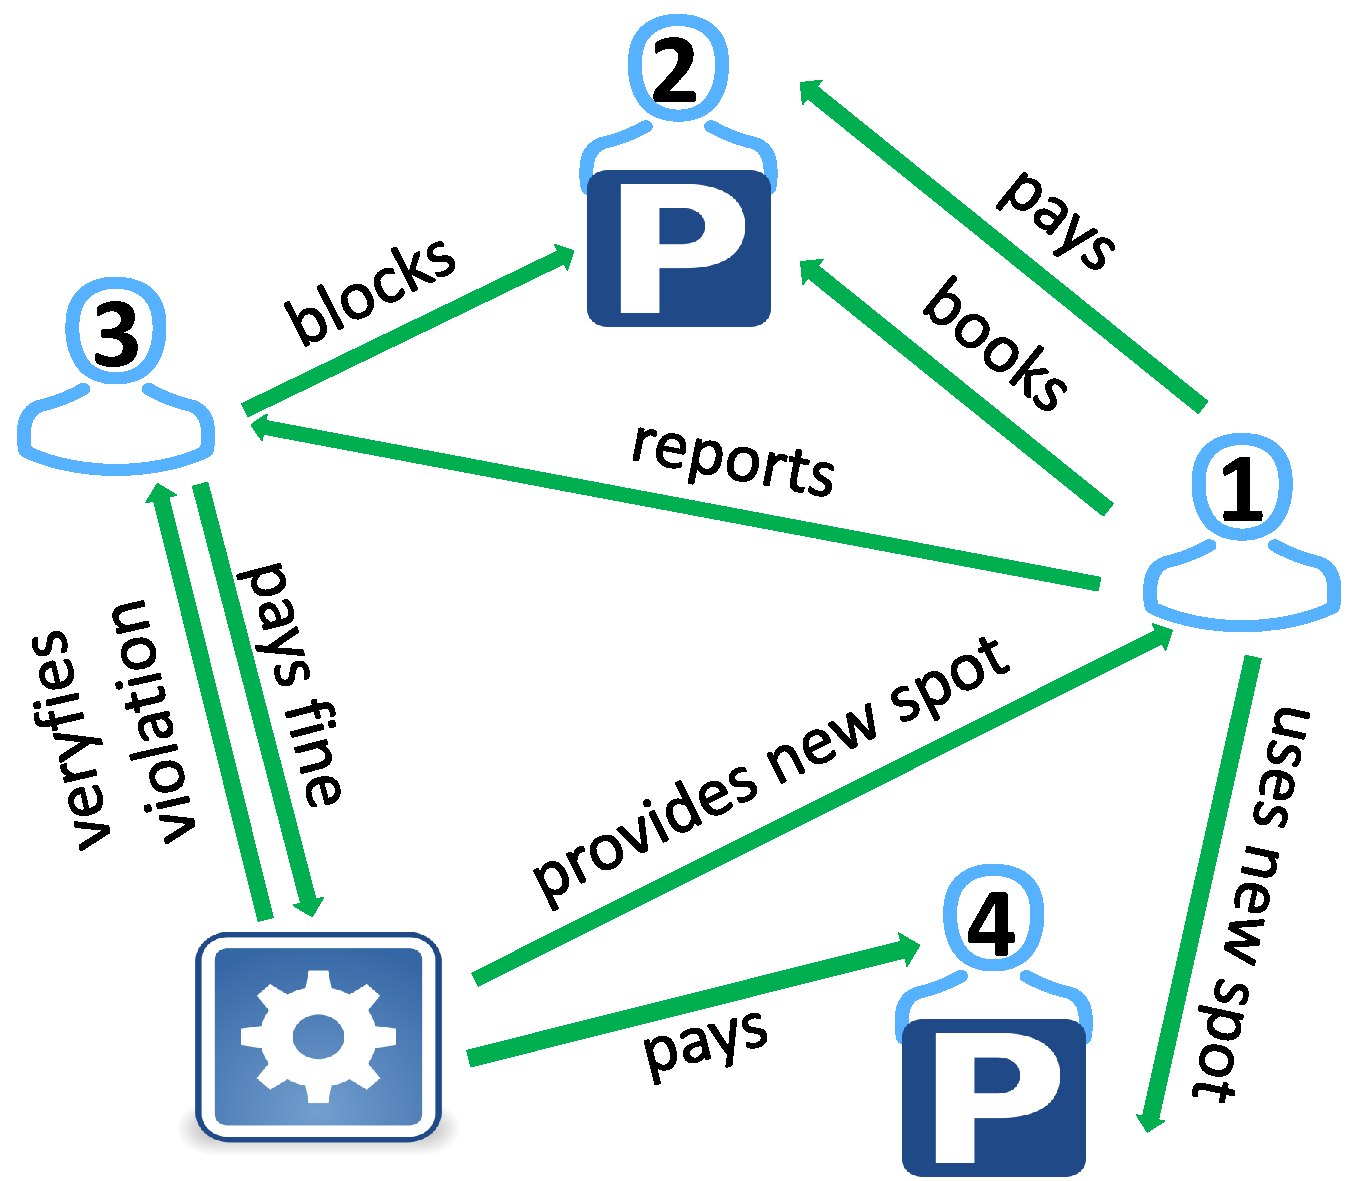
\includegraphics[width=13cm,height=11cm]{example_grafik.pdf}
	\caption{A possible example for the handling of rule violations}
	\label{img:example-grafik}
\end{figure}
 
Of course, it is also conceivable that user 3 has not occupied the parking space at all, but user 1 still reports him. In this case, the verifiers will report that the parking space is actually free. Now the system penalizes user 1 with a sum that covers the costs for the newly allocated parking space (of user 4) and the costs for the verifying users.\\

Another possibility is that user 3 has actually occupied the parking lot but has already left until the users arrive for verification. In this case, like above, the system would identify user 1 as the scammer, although user 3 violated the rules. It also imposes the fine on User 1. He now has the opportunity to challenge the fine. If he does, the confidence score comes into play. If both users are new users or neither of them has a particularly bad or good score, no fair decision can really be made and the costs incurred are borne by the system. In all other cases, when one user is clearly more trustworthy than another, the system decides in favour of the more trustworthy user.


\section{Security Analysis}

\section{Implementation}
The system is implemented according to the client-server model. Users utilize a smart phone as a client, while the operator provides a server on which a central database is hosted. Also running on the server is a web service that can be requested by the clients via a REST API. The web sercive forwards the request to the database system and also returns the response back to the clients. An Android app was developed for the clients using Java. The web service is also written in Java and runs on a Tomcat server, while a MySQL server has been set up for the database system.

\section{Future Work}

\section{Conclusion}

\section{Acknowledgments}
I would like to thank Prof. Dr. Alexandra Dmitrienko and the city of Würzburg, who both supported me in creating this work.















%%%
%%% end main document
%%%
%%%%%%%%%%%%%%%%%%%%%%%%%%%%%%%%%%%%%%%%%%%%%%%%%%%%%%%%%%%%%%%%%%%%%%%%%%%%%%%%

% \appendix  %% include it, if something (bibliography, index, ...) follows below

%%%%%%%%%%%%%%%%%%%%%%%%%%%%%%%%%%%%%%%%%%%%%%%%%%%%%%%%%%%%%%%%%%%%%%%%%%%%%%%%
%%%
%%% bibliography
%%%
%%% available styles: abbrv, acm, alpha, apalike, ieeetr, plain, siam, unsrt
%%%
% \bibliographystyle{plain}

%%% name of the bibliography file without .bib
%%% e.g.: literatur.bib -> \bibliography{literatur}
% \bibliography{FIXXME}

\end{document}
%%% }}}
%%% END OF FILE
%%%%%%%%%%%%%%%%%%%%%%%%%%%%%%%%%%%%%%%%%%%%%%%%%%%%%%%%%%%%%%%%%%%%%%%%%%%%%%%%
%%% Notice!
%%% This file uses the outline-mode of emacs and the foldmethod of Vim.
%%% Press 'zi' to unfold the file in Vim.
%%% See ':help folding' for more information.
%%%%%%%%%%%%%%%%%%%%%%%%%%%%%%%%%%%%%%%%%%%%%%%%%%%%%%%%%%%%%%%%%%%%%%%%%%%%%%%%
%% Local Variables:
%% mode: outline-minor
%% OPToutline-regexp: "%% .*"
%% OPTeval: (hide-body)
%% emerge-set-combine-versions-template: "%a\n%b\n"
%% End:
%% vim:foldmethod=marker
